\chapter{Introduction}
\label{ch:1}
%\setcounter{page}{1}
\pagenumbering{arabic}

\bigskip
\bigskip
\bigskip

This chapter presents the introduction of the thesis that includes the brief description of the purpose of the project, the problem being investigated, the background of the problem, previous works, our thesis and general approach and the criteria of success.

We are at a point of time where electronic devices like mobile phones and computers with internet connection become an important part of our daily life. The social media platforms are the main spreading source of the media files (image, audio or video). The amount of media files in the world is continously increasing. The social media platforms gets and shows these media contents but does not verify the originality of the content. This makes it very important to be able to verify online image content specially when and by whom it was captured, what was the geo location, is the image edited, if yes by whom, when and other information.

A news channel or a news feed in a social media platform, is a place where different informative media are shown to the world. People come to the social media platform to see what is other's status in the news feed.

In the context of unaccredited news, some videos have been manipulated or the image taken out of its context. This thesis investigates methods to verify image content based on a specific criteria: integrity (i.e., non-modification) of the recording. This would not only flag as unverified a lot of fake news images but might also be used to give increased credibility to images which can be verified.

This chapter gives a brief introduction to this thesis.
Section \ref{sec:background} gives a general background to the reader.
Section \ref{sec:problem} further discusses the problems that this thesis will investigate.
Section \ref{sec:purpose} gives a brief overview of our ideas regarding how the problem will be solved and why.
Section \ref{sec:goals} succinctly breaks down and quantizes the project into measurable goals.
Section \ref{sec:methods} presents a general framework and approach to the complete project.
Section \ref{sec:setup} explains the initial idea regarding what the final proof of concept prototype will look like.
In Section \ref{sec:boundary} the delimitations are discussed and why certain areas have been excluded.
Finally, Section \ref{sec:structure} outlines the entirety of this thesis.

\section{Background}
\label{sec:background}
Image integrity is the task of checking if the image file's bits are changed or not at any point. A digital file might change by platforms. This would be fully online system. Nowadays with increasing people in digital world the editing softwares are getting smart. Most of the files that might be non-editable in some operating systems or file systems, but the so called hackers or masters of electronic devices have file systems that can easily access and change any file data. So in that way the media files can not be checked for integrity. And also while the images are shared in different platforms, the files' data might be changed a little bit according to their protocols for data compression or security. Online platforms or social media just use public data, but they neither care about the originality of the data, nor there exists a fixed verification process for it.

The topic of this thesis is, as previously mentioned, highly relevant and widely discussed but usually not in the context of blockchains. Blockchain technology has the potential to provide data security and enable validation of the integrity of the data

The proposed system in this thesis will help us to detect those shared files and compare them not bit by bit, but context wise and signature wise. That means if one shares an image both our system as well as one of those online platforms and download them as separate file and check in our system, it should return truth values if data portion are same or atleast 95\% same. The system we are introducing the social media like platform that have the capability to store images and show them in news feed. There is a option for every photo to download in user's computer or mobile devices and after sharing and getting back the person can check if the file is intact or not in our proposed system by the digital signature.

\section{Problem}
\label{sec:problem}
More and more electronic devices like mobile phones and computers are equipped with cameras, internet connections, and verious sensors. The increasing capabilities of current devices enable the end user to produce and distribute media contents more easily than before. One issue that has arisen from this is the inability to be able to distinguish between a modified image and the original image. Additionally, images are taken out of context or claimed to be from a place and/or time different from what might actually be the truth. It is getting increasingly difficult for the viewer to know what to believe, who to believe, and tools to help counter these issues are rare and limited.

A service as proposed by this thesis will need to be trusted by its users. It is therefore of utmost importance to be able to ensure the integrity of the service and its software. The user needs to be able to trust the files they are downloading, and using on their devices. No additional software is required for the user to download except a reliable web-browser that very often comes with smartphone or computer.

\section{Purpose}
\label{sec:purpose}
The purpose of this thesis is to set up and evaluate the usage of a blockchain in order to verify and store signature hashes from live-captured image content as well as uploaded images from any device.
The creation of the signature hashes should be done as soon as the upload request comes, leaving as little time as possible for data manipulation by anyone and enabling the establishment of the precedence of this signed hash (\textit{i.e.}, it can be shown that it was signed at a particular period in time (based upon the entries before and after it in the blockchain), therefore the hash had to be calculated before this, and hence the media over which the hash is computed has to be even earlier than this).
In this thesis project, the signature hash is stored in a blockchain. Verification methods for these hashes are implemented
and accessible to users via a web-based interface. This proof of concept prototype showcases the potential of combining blockchains with hashes over chunks of media content and meets the requirements of the evolving world of streaming media content.

About all compression schemes says all the information of image is not useful we have to identify the useful regions of image and then try to integrate these regions of images. The objective why we write this thesis is If an  image in system then it is original but if it not in system System cannot confirm about it.

\section{Goals of the Thesis}
\label{sec:goals}
The measurable goals for this Thesis can be enumerate as three goals through which we aim to develop and evaluate a proof of concept prototype. The prototype when complete should be able to:
\begin{enumerate}
\item Determine whether an image has been taken at a specified time.
\item Determine which parts of the image whose integrity can/cannot be verified
\item The process of verifying the image through the entire blockchain should require less than 3 seconds.
\end{enumerate}

\section{Research Methodology}
\label{sec:methods}
The qualitative hypothetico-deductive method is used for this thesis. We have selected a deductive method since it uses previous theory and the main goal of the thesis is to prove a theory; specifically, to prove that blockchain technology is a suitable tool to ensure image integrity for any image. This is the hypothesis we wish to either confirm or dismiss.

We have chosen a qualitative method as this project is primary exploratory research within the combined areas of image integrity and blockchains. We seek to provide insights into the problem being investigated. The data collection method in this thesis will be unstructured and dependent upon the actual progress toward the project's goals.

The system that we are trying to build is capable of processing, storing and showing image files. Not only that, it also allows viewers to veryfy his own copy of the image. It is not easy to store and veryfy in a moment and it is about impossible to change the whole blockchain, because the miners have their own copy of the public ledger and their processed computation powers in their computers. The automated server should back up its data from both the Virtual miners as well as remote miners' computers. The studied and inspired technologies are discussed in the thesis.

The images collected during the investigation will be highly reliable since it will be collected by software without any human interaction. The image data is replicable as long as the same hardware and software are used. This is due to the fact that different hardware has different characteristics (such as processing power and read/write memory speed).

\section{Setup}
\label{sec:setup}
The system service (LAMPP web server) runs on a Dell Inspiron with Ubuntu Bionic Beaver (18.04.15). The client system is also in the same computer but the system we are building for a website that codes will be uploaded on a rermote dedicated linux web server.

The system can be seen in next figure. The decentralized web-application is built using PHP-7 (Personal Home Page or Hypertext PreProcessesor), CSS-3 (Cascading Style Sheets) and JS-5 (JavaScipt) language. PHP runs in server computer and JS runs in clients' browsers.

There are two phases of processing user image, i.e. whether the user wants to store image or verify image. So there are two separate page for these two. Moreover there are two different ways an user can request to store image, either by image uploadation or by web-camera. So we have separate page for that too.

\begin{figure}
\begin{center}
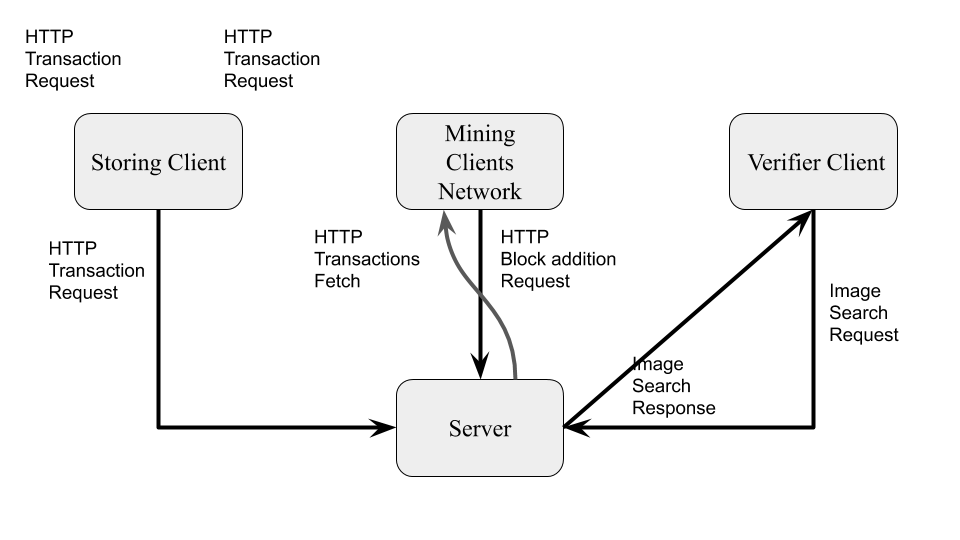
\includegraphics[width=\textwidth]{./img_src/setup.png}
\end{center}
\label{fig_setup}
\caption{Overview of Proposed System Model}
\end{figure}

\begin{figure}
\begin{center}
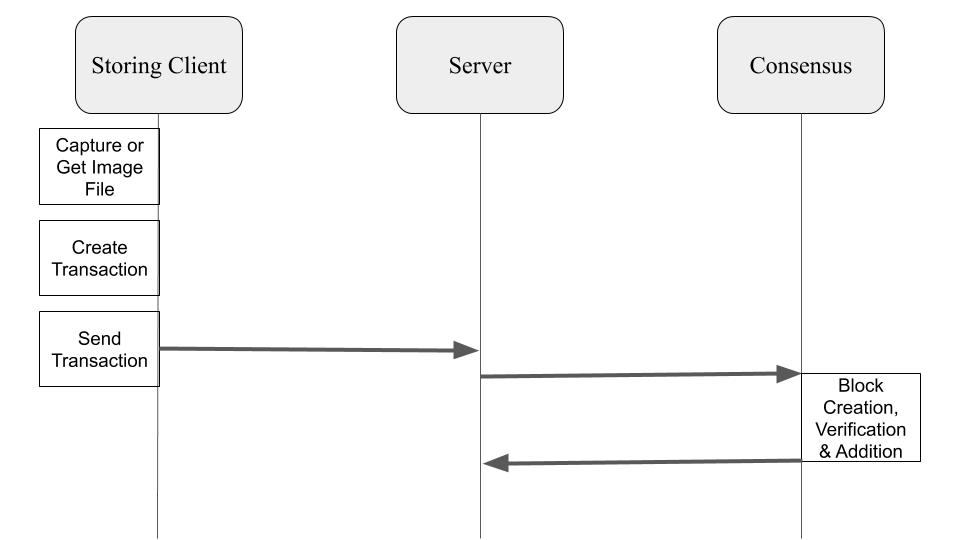
\includegraphics[width=\textwidth]{./img_src/img_store.png}
\end{center}
\label{fig_imgStore}
\caption{A process diagram for Image Insertion}
\end{figure}

\begin{figure}
\begin{center}
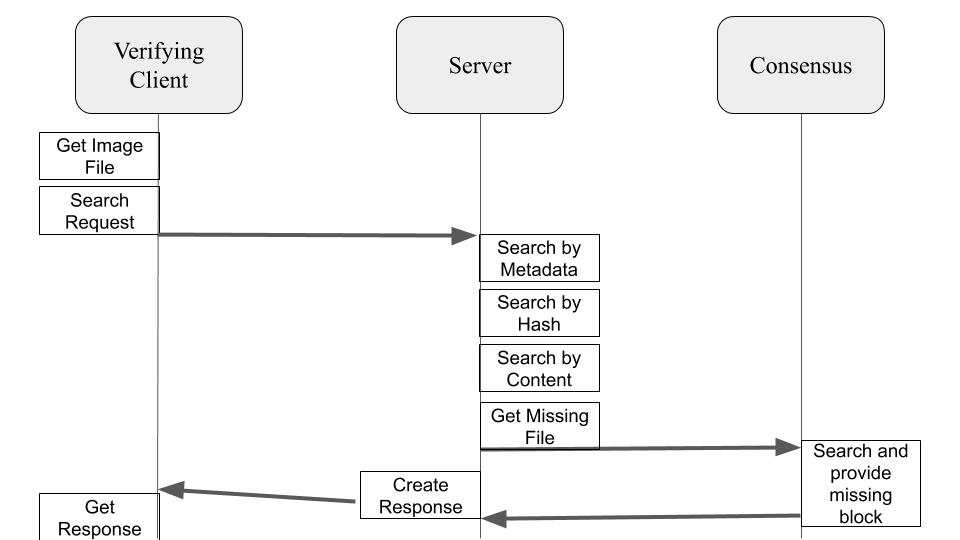
\includegraphics[width=\textwidth]{./img_src/img_verify.png}
\end{center}
\label{fig_imgVerify}
\caption{A process diagram for Image Verification}
\end{figure}

\section{Delimitations}
\label{sec:boundary}
This thesis will investigate and develop a proof of concept prototype showcasing the merger of an app running on an Android device with a backend security system using blockchain verification through smart contracts. However, the thesis will also examine what type of manipulation or tampering has been done to the recorded data, and it will simply verify if the hash of the image content is the same as that of the signed hash as recorded in the blockchain. There already exists a huge amount of methods for detecting data tampering and detecting what has actually been manipulated. The planned proof of concept prototype will simply determine whether or not the hash of the image subjected to verification matches the original image's hash saved by the client device in the blockchain. Additionally, the use of a blockchain is not limited here to setting up a working blockchain which can handle and store unique hashes from connected Android devices.

Other delimitations are the assumption of a perfect connection between the client device and the server, \textit{i.e.}, without any data loss. This loss free communication is required for both the upload of the image to be compared and the upload of hashes (with the meta data) to the blockchain. The issue of handling packet-loss in these scenarios are outside of the scope of this thesis.

\section{Roadmap of the Thesis}
\label{sec:structure}
The structure of the thesis is as follows:
\begin{enumerate}
\item The Chapter \ref{ch:1} is an introductory part which discusses the scope of the thesis, about the contribution of this thesis and the motivation for writing it.
\item The Chapter \ref{ch:2} provides the background of Image integrity security aspects of it and previous works.
\item The detailed descrption of the proposed mechanism is discussed in Chapter \ref{ch:3}.
\item The implementation of Chapter \ref{ch:4}, where an informal implementation of the proposed protocol has been discussed.
\item The Chapter \ref{ch:5} comprises of the conclusion and further work of the Project in future.
\item The Final Chapter is the Appendix \textit{i.e.} the detaied information of the technologies used as a combination model in this project.
\end{enumerate}

\section{Scope of Discussion}
This thesis focuses on building a hybrid architechture inspired by one of the major implementations of BlockChain i.e. BitCoin ~\cite{nakamoto2008bitcoin}. By the advancement of PHP (Hypertext PreProcessor) and JS (JavaScript) which are the basic web building languages or platforms that can be run in any modern devices, it might be quite easy to make a peer-to-peer web-api (Application Programming Interface) running like bitcoin decentraized network as well as social media platform that might be a real Truth Machine. While comparing image files data we will first compress the data using our own protocol and compare by bit matching Euclid, or Deep CNN (Convolutional Neural Network).

\section{Thesis Contribution}
The main contributions of this thesis includes
\begin{enumerate}
\item Proposes an user anonymity-preserving algorithm to be a part of Image Integrity Program.
\item Formally analyzes the security of the newly designed protocol as well as its performance.
\item The scheme, as compared to the existing schemes, not only authenticates the users but, also establishes a session key between the user and the System after successful mutual authentication.
\item The scheme provides many security and robustness features of user authentication and Block Processing scheme for BCTs.
\item No installation required to be a part of the system, except you want to be the miner.
\end{enumerate}
